\begin{minipage}{0.55\textwidth}
\begin{align*}
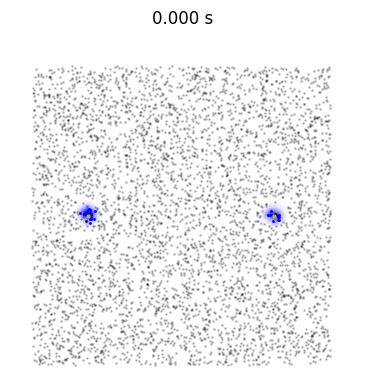
\includegraphics[width=0.49\textwidth]{simulation/7/frame_0.png}\hfill
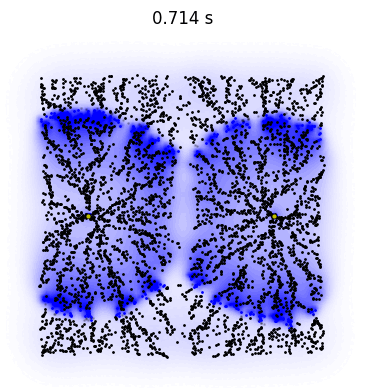
\includegraphics[width=0.49\textwidth]{simulation/7/frame_119.png}
\\[\smallskipamount]
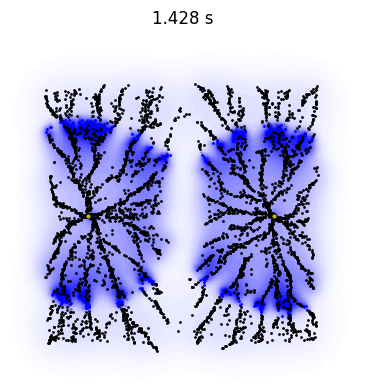
\includegraphics[width=0.49\textwidth]{simulation/7/frame_238.png}\hfill
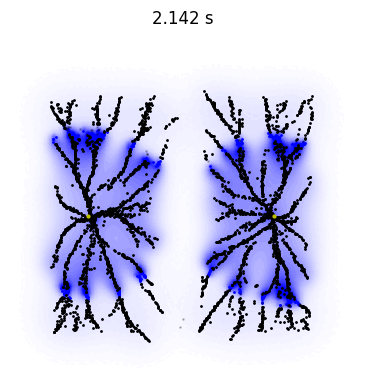
\includegraphics[width=0.49\textwidth]{simulation/7/frame_357.png}
\\[\smallskipamount]
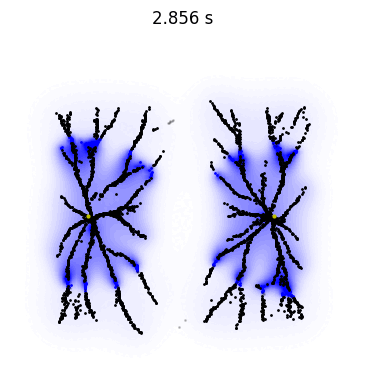
\includegraphics[width=0.49\textwidth]{simulation/7/frame_476.png}\hfill
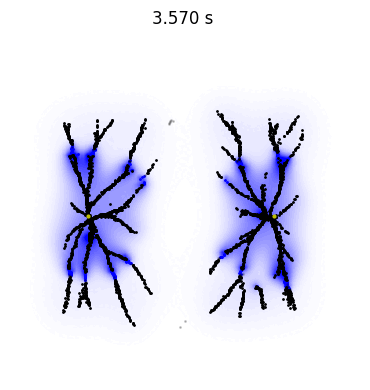
\includegraphics[width=0.49\textwidth]{simulation/7/frame_595.png}
\\[\smallskipamount]
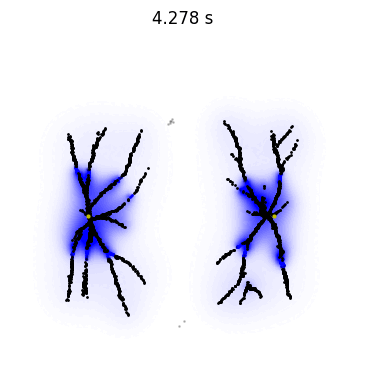
\includegraphics[width=0.49\textwidth]{simulation/7/frame_713.png}\hfill
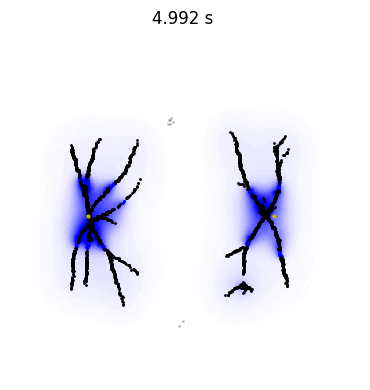
\includegraphics[width=0.49\textwidth]{simulation/7/frame_832.png}
\end{align*}
\end{minipage}
\begin{minipage}{0.45\textwidth}
\subsection{In Sync Pacemakers}
Here we tried a uniform distribution on a square but having two pacemakers which are running in sync.
One can observe that similar to the case of the Annulus we have a clear separation where the two concentration fronts collide.
This leads to a clear and straight separation of the two structures which are of a similar size.
\end{minipage}